\documentclass[12pt]{article}
\usepackage[danish]{babel}
\usepackage{amsfonts, amssymb, mathtools, amsthm, amsmath}
\usepackage{graphicx, pgfplots}
\usepackage{url}
\usepackage[dvipsnames]{xcolor}
\usepackage{sagetex}
\usepackage{lastpage}
\usepackage[stretch=10]{microtype} 

%loaded last
\usepackage[hidelinks]{hyperref}

\usepackage{siunitx}
  \sisetup{exponent-product = \cdot,
    output-decimal-marker = {,}}

%Giles Castelles incfig
\usepackage{import}
\usepackage{xifthen}
\usepackage{pdfpages}
\usepackage{transparent}

\newcommand{\incfig}[2][1]{%
  \def\svgwidth{#1\columnwidth}
  \import{../figures/}{#2.pdf_tex}
}

\setlength{\parindent}{0in}
\setlength{\oddsidemargin}{0in}
\setlength{\textwidth}{6.5in}
\setlength{\textheight}{8.8in}
\setlength{\topmargin}{0in}
\setlength{\headheight}{18pt}

\usepackage{fancyhdr}
\pagestyle{fancy}

\fancyhead{}
\fancyfoot{}
\fancyfoot[R]{Side \thepage{} af \pageref{LastPage}}
\fancyhead[C]{\leftmark}

\pgfplotsset{compat=newest}

\pgfplotsset{every axis/.append style={
  axis x line=middle,    % put the x axis in the middle
  axis y line=middle,    % put the y axis in the middle
  axis line style={<->,color=black}, % arrows on the axis
}}

\usepackage{thmtools}
\usepackage{tcolorbox}
  \tcbuselibrary{skins, breakable}
  \tcbset{
    space to upper=1em,
    space to lower=1em,
  }

\theoremstyle{definition}

\newtcolorbox[auto counter]{definition}[1][]{%
  breakable,
  colframe=ForestGreen,  %frame color
  colback=ForestGreen!5, %background color
  colbacktitle=ForestGreen!25, %background color for title
  coltitle=ForestGreen!70!black,  %title color
  fonttitle=\bfseries\sffamily, %title font
  left=1em,              %space on left side in box,
  enhanced,              %more options
  frame hidden,          %hide frame
  borderline west={2pt}{0pt}{ForestGreen},  %display left line
  title=Definition \thetcbcounter: #1,
}

\newtcolorbox{greenline}{%
  breakable,
  colframe=ForestGreen,  %frame color
  colback=white,          %remove background color
  left=1em,              %space on left side in box
  enhanced,              %more options
  frame hidden,          %hide frame
  borderline west={2pt}{0pt}{ForestGreen},  %display left line
}

\newtcolorbox[auto counter, number within=section]{eks}[1][]{%
  brekable,
  colframe=NavyBlue,  %frame color
  colback=NavyBlue!5, %background color
  colbacktitle=NavyBlue!25,    %background color for title
  coltitle=NavyBlue!70!black,  %title color
  fonttitle=\bfseries\sffamily, %title font
  left=1em,            %space on left side in box,
  enhanced,            %more options
  frame hidden,        %hide frame
  borderline west={2pt}{0pt}{NavyBlue},  %display left line
  title=Eksempel \thetcbcounter: #1
}

\newtcolorbox{blueline}{%
  breakable,
  colframe=NavyBlue,     %frame color
  colback=white,         %remove background
  left=1em,              %space on left side in box,
  enhanced,              %more options
  frame hidden,          %hide frame
  borderline west={2pt}{0pt}{NavyBlue},  %display left line
}

\newtcolorbox{teo}[1][]{%
  breakable,
  colframe=RawSienna,  %frame color
  colback=RawSienna!5, %background color
  colbacktitle=RawSienna!25,    %background color for title
  coltitle=RawSienna!70!black,  %title color
  fonttitle=\bfseries\sffamily, %title font
  left=1em,              %space on left side in box,
  enhanced,              %more options
  frame hidden,          %hide frame
  borderline west={2pt}{0pt}{RawSienna},  %display left line
  title=Teori: #1,
}

\newtcolorbox[auto counter, number within=section]{sæt}[1][]{%
  breakable,
  colframe=RawSienna,  %frame color
  colback=RawSienna!5, %background color
  colbacktitle=RawSienna!25,    %background color for title
  coltitle=RawSienna!70!black,  %title color
  fonttitle=\bfseries\sffamily, %title font
  left=1em,              %space on left side in box,
  enhanced,              %more options
  frame hidden,          %hide frame
  borderline west={2pt}{0pt}{RawSienna},  %display left line
  title=Sætning \thetcbcounter: #1,
  before lower={\textbf{Bevis:}\par\vspace{0.5em}},
  colbacklower=RawSienna!25,
}

\newtcolorbox{redline}{%
  breakable,
  colframe=RawSienna,  %frame color
  colback=white,       %Remove background color
  left=1em,            %space on left side in box,
  enhanced,            %more options
  frame hidden,        %hide frame
  borderline west={2pt}{0pt}{RawSienna},  %display left line
}

\newtcolorbox{for}[1][]{%
  breakable,
  colframe=NavyBlue,  %frame color
  colback=NavyBlue!5, %background color
  colbacktitle=NavyBlue!25,    %background color for title
  coltitle=NavyBlue!70!black,  %title color
  fonttitle=\bfseries\sffamily, %title font
  left=1em,              %space on left side in box,
  enhanced,              %more options
  frame hidden,          %hide frame
  borderline west={2pt}{0pt}{NavyBlue},  %display left line
  title=Forklaring #1,
}

\newtcolorbox{bem}{%
  breakable,
  colframe=NavyBlue,  %frame color
  colback=NavyBlue!5, %background color
  colbacktitle=NavyBlue!25,    %background color for title
  coltitle=NavyBlue!70!black,  %title color
  fonttitle=\bfseries\sffamily, %title font
  left=1em,              %space on left side in box,
  enhanced,              %more options
  frame hidden,          %hide frame
  borderline west={2pt}{0pt}{NavyBlue},  %display left line
  title=Bemærkning:,
}

\makeatother
\def\@lecture{}%
\newcommand{\lecture}[3]{
  \ifthenelse{\isempty{#3}}{%
    \def\@lecture{Lecture #1}%
  }{%
    \def\@lecture{Lecture #1: #3}%
  }%
  \subsection*{\makebox[\textwidth][l]{\@lecture \hfill \normalfont\small\textsf{#2}}}
}

\makeatletter

\newcommand{\opgave}[1]{%
 \def\@opgave{#1}%
 \subsection*{Opgave #1}
}

\makeatother

%Format lim the same way in intext and in display
\let\svlim\lim\def\lim{\svlim\limits}

% horizontal rule
\newcommand\hr{
\noindent\rule[0.5ex]{\linewidth}{0.5pt}
}

\title{Afleveringsopgave nr. 5}
\author{Noah Rahbek Bigum Hansen}
\date{7. November 2024}

\begin{document}

\maketitle

\section*{Problem 1/3}
I indledningssekvensen i filmen ``Rumrejse år 2001'' ses en astronaut under sin morgenmotion. I en torusformet rumstation, der langsomt roterer om toroidens symmetriakse løber astronauten rundt på stationens ``gulv''. Antag at toroidens diameter er \qty{20}{m}, og at rotationen frembringer et effektivt tyngdefelt på \qty{5}{m/s^2}.

\begin{figure}[ht]
  \centering
  \incfig[0.4]{A1P1}
  \caption{Fritlegemediagram for rumstationen og astronauten.}
  \label{fig:A1P1}
\end{figure}

\subsection*{(a)}
Bestem rumstationens vinkelhastighed.
\bigbreak
Den oplevede tyngdekraft for astronauten må netop tilsvare den normalkraft som astronauten oplever. Vi har desuden at det eneste bidrag til normalkraften $N$ er centripetalkraften $F_{cp}$ så vi har at

\begin{equation} \label{eq:fcp}
  F_{g_{eff}} = N = F_{cp}
\end{equation}

Dette må betyde at den oplevede tyngdeacceleration netop må tilsvare centripetalaccelerationen så

\begin{equation} \label{eq:cpacc}
  g_{eff} = a_{rad} = \omega^2\cdot r
\end{equation}

Vi isolerer vinkelhastigheden $\omega$ i ovenstående
\[ 
\omega = \sqrt{\frac{g_{eff}}{r}} = \sqrt{\frac{\qty{5,00}{\frac{m}{s^2}}}{\qty{10}{m}}} = \qty{0,707}{\frac{rad}{s}} 
.\]
Altså skal rumstationen have en vinkelhastighed på  \underline{\underline{\qty{0,7}{rad/s}}}.


\subsection*{(b)}
Bør astronauten løbe ``med'' eller ``mod'' rotationsretningen for at få mest motion?
\bigbreak
Af \autoref{eq:cpacc} ses at den centripetale acceleration stiger, hvis vinkelhastigheden stiger. Astronautens vinkelhastighed vil, hvis han bevæger sig, være summen af vinkelhastigheden for hans eget løb rundt i rumstationen og rumstationens bevægelse. Altså vil astronautens samlede vinkelhastighed blive større, hvis han løber ``med'' rumstationen rundt i bevægelsen. Eftersom astronauten får en større vinkelhastighed ved at løbe ``med'' rumstationen rundt må han også opleve en større centrifugalkraft og løbet vil derfor være hårdere for ham, idet det oplevede tyngdefelt ville være større.
\bigbreak
\underline{\underline{Altså skal astronauten løbe ``med'' rumstationen rundt for at få mest motion.}}


\subsection*{(c)}
Hvad er den maksimale hastighed astronauten kan benytte, hvis han løber ``mod'' rotationsretningen, og hvad sker der, hvis han løber hurtigere? 
\bigbreak
Astronauten vil (teoretisk set) være i stand til at løbe indtil at han løber netop så stærkt, at den oplevede tyngdekraft $F_{g_{eff}}$ bliver 0 idet han her netop vil blive vægtløs. Fra \autoref{eq:fcp} har vi at $F_{g_{eff}} = F_{cp}$. Altså har vi at
\[ 
  F_{g_{eff}} = F_{cp} = m\omega^2 \cdot r = 0 \implies \omega = 0
.\]
Vi skal altså finde et udtryk for astronautens vinkelhastighed, $\omega_a$, som funktion af hans tangentielle hastighed, $v_a$. Tangentiel hastighed er blot produktet af vinkelhastighed og radius, så
\[ 
v_{a} = r\cdot \omega_{a}
.\]
Vi ønsker at finde astronautens hastighed netop hvor summen af vinkelhastighederne $|\omega_a| - |\omega| = 0$, så
\[ 
  v_{a_{maks}} = r \cdot \omega = \qty{10}{m} \cdot \qty{0,707}{\frac{rad}{s}}  = \qty{7,07}{\frac{m}{s}}  
.\]
Altså kan astronauten maksimalt løbe med \underline{\underline{\qty{7}{m/s}}} før han bliver vægtløs. 
\bigbreak
Det bør dog bemærkes, at astronauten i praksis ikke ville kunne nå denne hastighed, da løb nok bliver umuligt for tilpas lave værdier af $F_{g_{eff}}$. Får astronauten på en eller anden måde accelereret sig så han kommer til at løbe hurtigere end $v_{a_{maks}}$ så vil han blive vægtløs netop når $v_a = v_{a_{maks}}$ og for $v_{a_{maks}}<v_a$ vil astronauten give sig selv en ny centripetalkraft som vil blive kraftigere i takt med at hans hastighed stiger ift. $v_{a_{maks}}$.

\section*{Problem 2/3}
A \qty{500,0}{g} bird is flying horizontally at \qty{2,25}{m/s}, not paying much attention, when it suddenly flies into a stationary vertical bar, hitting it \qty{25,0}{cm} below the top (\textbf{\autoref{fig:A1P1}}). The bar is uniform, \qty{0,750}{m} long, has a mass of \qty{1,50}{kg}, and is hinged at its base. The collision stuns the bird so that it just drops to the ground afterward (but soon recovers to fly happily away). What is the angular velocity of the bar

\begin{figure}[ht]
  \centering
  \incfig[0.4]{A1P2}
  \caption{Skitsering af situationen, hvor fuglen flyver ind i stangen.}
  \label{fig:A1P2}
\end{figure}

\subsection*{(a)}
just after it is hit by the bird and
\bigbreak
Før kollisionen er det kun fuglen, der bevæger sig. Dennes impulsmoment omkring hængslet er
\[ 
L_0 = m_f v_f r
,\]
hvor $m_f$ er fuglens masse, $v_f$ er fuglens hastighed og $r = \qty{0,50}{cm}$ er afstanden fra det punkt fuglen rammer til hængslet. Efter kollisionen er al bevægelsen overført til baren således, at det kun er stangens rotation, der bidrager til det samlede impulsmoment. Impulemomentet efter kollisionen må derfor være lig stangens impulsmoment
\[ 
L_1 = I_s\omega_1
,\]
hvor $I_s$ er stangens inertimoment. Idet impulsmoment er en konserveret størrelse må det gælde at
\[ 
L_0 = L_1 \implies \omega_1 = \frac{m_fv_fr}{I} 
.\]
Stangen modelleres som en tynd cylinder og dens inertimoment er derfor
\[ 
  I_{s} = \frac{1}{3} ML_s^2 = \frac{1}{3} \cdot \qty{1,50}{kg} \cdot (\qty{0,750}{m})^2 = \qty{0,28125}{m^2.kg} 
.\]
Nu er alle størrelser fundet og vi kan derfor indsætte i udtrykket for vinkelhastigheden $\omega_1$
\[ 
\omega_1 = \frac{\qty{500,0}{g} \cdot \qty{2,25}{\frac{m}{s}} \cdot \qty{0,50}{cm}}{\qty{0,28125}{m^2.kg}} = \qty{2,00}{\frac{rad}{s}} 
.\]
Altså vil stangen netop efter fuglen har ramt den have en vinkelhastighed på \underline{\underline{\qty{2,00}{rad/s}}}. 


\subsection*{(b)}
just as it reaches the ground?
\bigbreak
Efter fuglen har ramt stangen er den eneste kraft der virker på den inden den rammer jorden tyngdekraften. Idet stangens masse er jævnfordelt og at stangen står op netop idet fuglen rammer den må dens massemidtpunkt i starten være placeret i en højde på
\[ 
h_{cm_0} = \frac{L_s}{2} = \qty{0,375}{m} 
.\]
Når stangen ligger ned er dens massemidtpunkt placeret i en højde på $h_{cm_1} = 0$, idet den antages at være uendeligt tynd. Derfor falder stangens massemidtpunkt i alt
\[ 
\Delta h_{cm} = h_{cm_0} - h_{cm_1} = \qty{0,375}{m} - 0 = \qty{0,375}{m}
.\]
Derfor må det samlede fald i potentiel energi være
\[ 
U_g = m_sg\Delta h_{cm} = \qty{1,50}{kg} \cdot \qty{0,375}{m}  \cdot g = \qty{5,5125}{J} 
.\]
Idet det antages at der ikke er nogen friktion eller luftmodstand må al denne potentielle energi omdannes til rotationel energi i stangen. Altså vil stangen opleve en tilvækst i rotationel energi på \qty{5,5125}{J}. Vi finder den rotationelle energi før tyngdekraften virker på stangen
\[ 
k_{rot_0} = \frac{1}{2}I_s\omega_1^2 = \frac{1}{2} \cdot \qty{0,28125}{m^2.kg} \cdot (\qty{2}{\frac{rad}{s}} )^2 = \qty{0,5625}{J} 
.\]
Den samlede rotationelle energi idet stangen rammer jorden må da være
\[ 
k_{rot_1} = U_g + k_{rot_0} = \qty{0,5625}{J} + \qty{5,5125}{J} = \qty{6,075}{J} 
.\]
Dette kan omregnes til en vinkelhastighed ved at isolere vinkelhastigheden i formlen for rotationsenergi
\[ 
  \omega = \sqrt{\frac{2k_{rot_1}}{I}} = \sqrt{\frac{2\cdot \qty{6,075}{J}}{\qty{0,28125}{m^2.kg}}} = \qty{6,57}{\frac{rad}{s}} 
.\]
Altså vil baren idet den rammer jorden have en vinkelhastighed på \underline{\underline{\qty{6,57}{rad/s}}}.





\section*{Problem 3/3}
A block with mass $m$ is revolving with linear speed $v_1$ in a circle of radius $r_1$ on a frictionless horizontal surface (see \textbf{\autoref{fig:AP3}}). The string is slowly pulled from below until the radius of the circle in which the block is revolving is reduced to $r_2$.

\begin{figure} [ht]
  \centering
  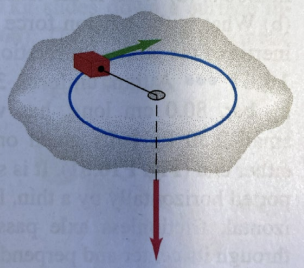
\includegraphics[width=0.5\linewidth]{../figures/AP3.png}
  \caption{Skitsering af situationen, hvor blokken roterer i en bane defineret af længden på snoren}
  \label{fig:AP3}
\end{figure}

\subsection*{(a)}
Calculate the tension $T$ in the string as a function of $r$, the distance of the block from the hole. Your answer will be in terms of the initial velocity $v_1$ and the radius $r_1$.
\bigbreak
Idet snoren holder klodsen i en cirkelbevægelse må spændingen $T$ i snoren netop tilsvare centripetalkraften $F_{cp}$. Vi har altså at
\[ 
T = F_{cp}
.\]
Idet snoren bliver trukket ind således at klodsen øger sin hastighed vil der være konservation af impulsmoment. Impulsmomentet er generelt givet som
\[ 
L = mrv
.\]
Og idet impulsmoment er konserveret må det gælde at
\[ 
m r_1 v_1 = m r_2 v_2 \implies v_2 = \frac{r_1v_1}{r_2}
.\]
Idet snoren holder klodsen i en cirkelbevægelse må spændingen $T$ i snoren netop tilsvare centripetalkraften $F_{cp}$. Vi har altså at
\[ 
T = \frac{v^2m}{r} = \frac{r_1^2v_1^2m}{r_2^3}
.\]
Altså er vores funktion $\underline{\underline{T(r) = \frac{r_1^2v_1^2m}{r^3}}}$.



\subsection*{(b)}
Use $W = \int_{r_1}^{r_2} \Vec{T}(r) \cdot \, \mathrm{d}\Vec{r}$ to calculate the work done by $\Vec{T}$ when $r$ changes from $r_1$ to $r_2$.
\bigbreak
Fra del (a) har vi funktionen
\[ 
T(r) = \frac{r_1^2v_1^2m}{r^3}
.\]
Vi ønsker at finde arbejdet vha. integralet. Dog skal vi huske at sætte nyt fortegn på det givne integrale idet, at der for konserverede krafter gælder at $-W = \int F \, \mathrm{d}r$. Altså
\[ 
W = -\int_{r_1}^{r_2} T(r) \, \mathrm{d}r 
.\]
Integralet beregnes ved først at faktorisere konstanterne ud og derefter finde integralet af det tilbageværende polynomium
\begin{align*}
  -\int_{r_1}^{r_2} \frac{r_1^2v_1^2m}{r^3} \, \mathrm{d}r &= -r_1^2v_1^2m \int_{r_1}^{r_2} r^{-3} \, \mathrm{d}r \\
  &= -r_1^2v_1^2m \cdot \left[ -\frac{1}{2r^2} \right]_{r_1}^{r_2} \\
  &= -\left( \frac{1}{2r_1^2} - \frac{1}{2r_2^2} \right)\cdot r_1^2v_1^2m \\
.\end{align*}
Altså har vi at spændingen i snoren $T$ udfører et arbejde på $\underline{\underline{W = - \left( \frac{1}{2r_1^2} - \frac{1}{2r_2^2} \right) \cdot r_1^2v_1^2m }}$


\subsection*{(c)}
Compare the results of part (b) to the change in the kinetic energy of the block.
\bigbreak
Den oprindelige kinetiske energi for blokken er
\[ 
k_1 = \frac{1}{2}mv_1^2
.\]
Og efter snoren har udført et arbejde kan vi finde den kinetiske energi idet vi husker at vi allerede har udledt et udtryk for hastigheden i denne situation $v_2$ i (a)
\[ 
k_2 = \frac{1}{2}mv_2^2 \implies \frac{1}{2} m \left( \frac{v_1r_1}{r_2} \right)^2 = \frac{1}{2}m  \frac{v_1^2r_1^2}{r_2^2}
.\]
Ændringen i kinetisk energi er derfor
\begin{align*}
  \Delta k &= k_2 - k_1 = \frac{1}{2}m \frac{v_1^2r_1^2}{r_2^2} - \frac{1}{2}mv_1^2 \\
  &= \frac{1}{2}mv_1^2 \left( \frac{r_1^2}{r_2^2}-1 \right) \\
  &= \frac{1}{2}mv_1^2r_1^2 \left( \frac{1}{r_2^2} - \frac{1}{r_1^2} \right)
.\end{align*}
Altså er det vist at ændringen i den kinetiske energi fundet ovenfor $\Delta k$ netop svarer til arbejdet $W$ fundet i (b).


\end{document}
